\documentclass[11pt]{article}
\usepackage{listings}
\usepackage{graphicx}
\usepackage{url}

\begin{document}

\begin{titlepage}
	\begin{center}
    	\includegraphics[scale=0.10]{du.png}\par
		\begin{Huge}
			\textsc{University of Dhaka}\par
		\end{Huge}
		\begin{Large}
			Department of Computer Science and Engineering\par \vspace{1cm}
			CSE-3111 : Computer Networking Lab \\[12pt]	
			Lab Report 2 : Introduction to Socket Programming using Java
		\end{Large}
	\end{center}  	
	\begin{large}
		\textbf{Submitted By:\\[12pt]}
			Name: Asfin Jannat Shamsi\\[8pt]
			Roll No : 23\\[12pt]
            Name: Tanzeem Maliat\\[8pt]
			Roll No : 51\\[12pt]
		\textbf{Submitted On : \\[12pt]}
			January 25, 2023\\[20pt]
		\textbf{Submitted To :\\[12pt]}
			Dr. Md. Abdur Razzaque\\[12pt]
                Md Mahmudur Rahman\\[12pt]
                Md. Ashraful Islam\\[12pt]
                Md. Fahim Arefin
	\end{large}
\end{titlepage}

\section{Introduction}
The preliminary object of this lab is to establish a TCP connection between Server and Client.This lab experiment was done a very basic one-way Client and Server setup where a Client connects, sends messages to the server and the server shows them using a socket connection. 

\subsection{Objectives}
The specific objectives of this lab experiment.
\begin{itemize}
    \item To establish a TCP connection between Server & Client
    \item To perform some operation by the Server process requested by the
Client and send responses from the Server
    \item To design and implement a non-idempotent operation
\end{itemize}
%%%%
%%%%
\section{Theory}
Socket Programming offers a very basic one-way Client and Server setup where a Client connects, sends messages to the server and the server shows them using a socket connection. The Java API networking package (java.net) takes care of all the low-level connections regarding the TCP, making network programming very easy for programmers.




\section{Checking Prime Number}
Here we will include the solve for the problem statement of checking if a number is prime or not given during the lab experiment.
\newpage
\subsection{Checking Prime Number Requested By The Client - Server Side }
This part contains the logical part to check whether a given number is prime or not along with the PrintStream object to send it over to the client side so that the client will see whether their given integer is a prime or not.
\lstinputlisting[language=java]{Server.java}

\begin{figure}[!h]
\centering
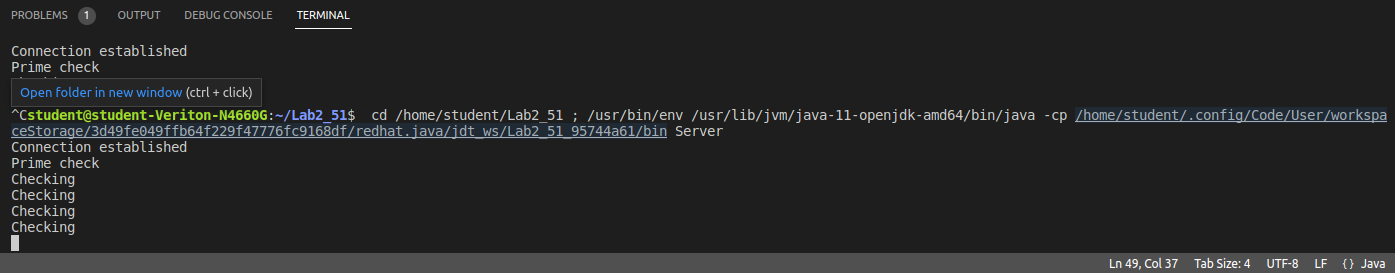
\includegraphics[width=\textwidth]{prime_server.png}
\caption{Server Side For The Prime Number Check}
\end{figure}
\newpage

\subsection{Checking The Prime Number Requested By The Client - Client Side}
Here our client side will establish a connection with the server. The client will send over an integer to check whether it is prime or not.  Then the logical part of the server side will output stream the result to the client and the statement will be shown over the client side

\lstinputlisting[language=java]{Client.java}

\begin{figure}[!h]
\centering
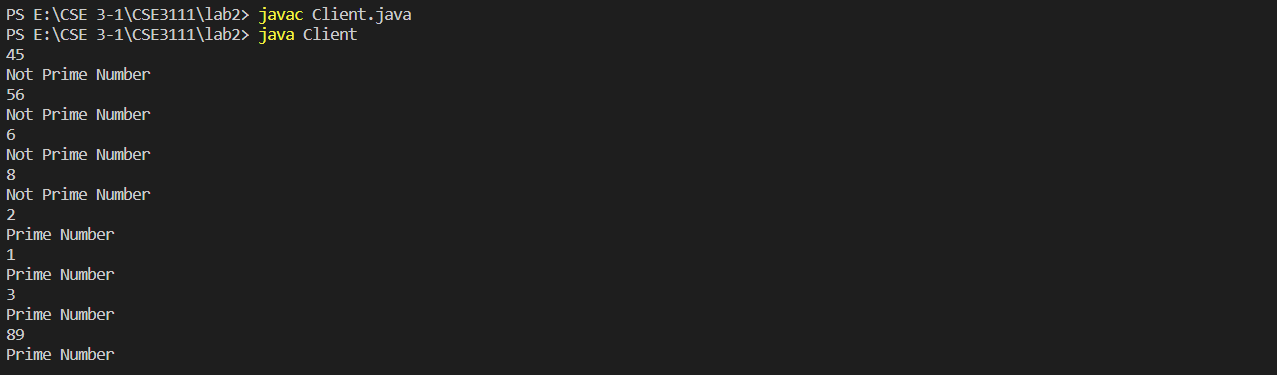
\includegraphics[width=\textwidth]{prime_client.png}
\caption{Client Side For The Prime Number Check}
\end{figure}
\newpage
\section{Letter Case Conversion}
Here we will include the solve for the problem statement of small letter to capital conversion for a line of text given during the lab experiment.
\subsection{Letter Case Conversion Requested By The Client - Server Side }
This section will show the part where the text received from the client side will be converted to capital letter along with small letter as an added line of code.
\lstinputlisting[language=java]{Server2.java}

\begin{figure}[!h]
\centering
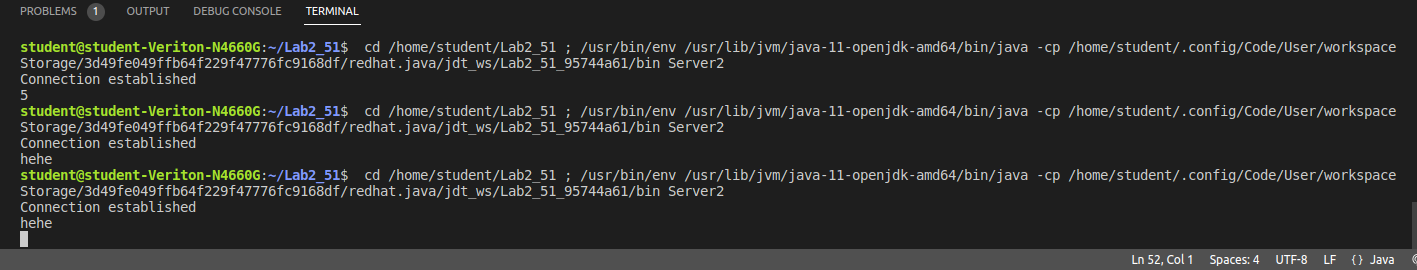
\includegraphics[width=\textwidth]{case_server.png}
\caption{Server Side For Letter Case Conversion}
\end{figure}


\subsection{Letter Case Conversion Requested By The Client - Client Side}
Here our client side will send over a text to the server & the output will be shown to the server both in all capital letters & smaller letters. 
\lstinputlisting[language=java]{Client2.java}

\begin{figure}[!h]
\centering
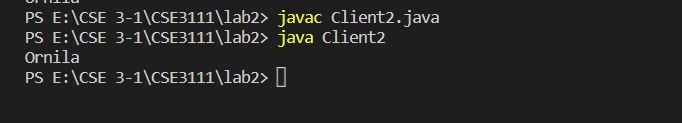
\includegraphics[width=\textwidth]{case_client.png}
\caption{Client Side For Letter Case Conversion}
\end{figure}

\section{A non-idempotent operation using exactly-once semantics handling failure of request messages, failure of response messages and process execution failures.}
Here we will include the solve for the problem statement of design and implementation a non-idempotent operation using exactly-once semantics that can handle failure of request messages, failure of response messages and process execution failures.given during the lab experiment.
\subsection{Handling Message Failure  Requested By The Client - Server Side }
This part will handle the registration of the user/client list. It will also control the balance, credit & debit part of one's transaction. A random number will be generated whose threshold above 70 will signal the failure of the data packet. This part can be enhanced using the graph. 
\lstinputlisting[language=java]{Server3.java}

\begin{figure}[!h]
\centering
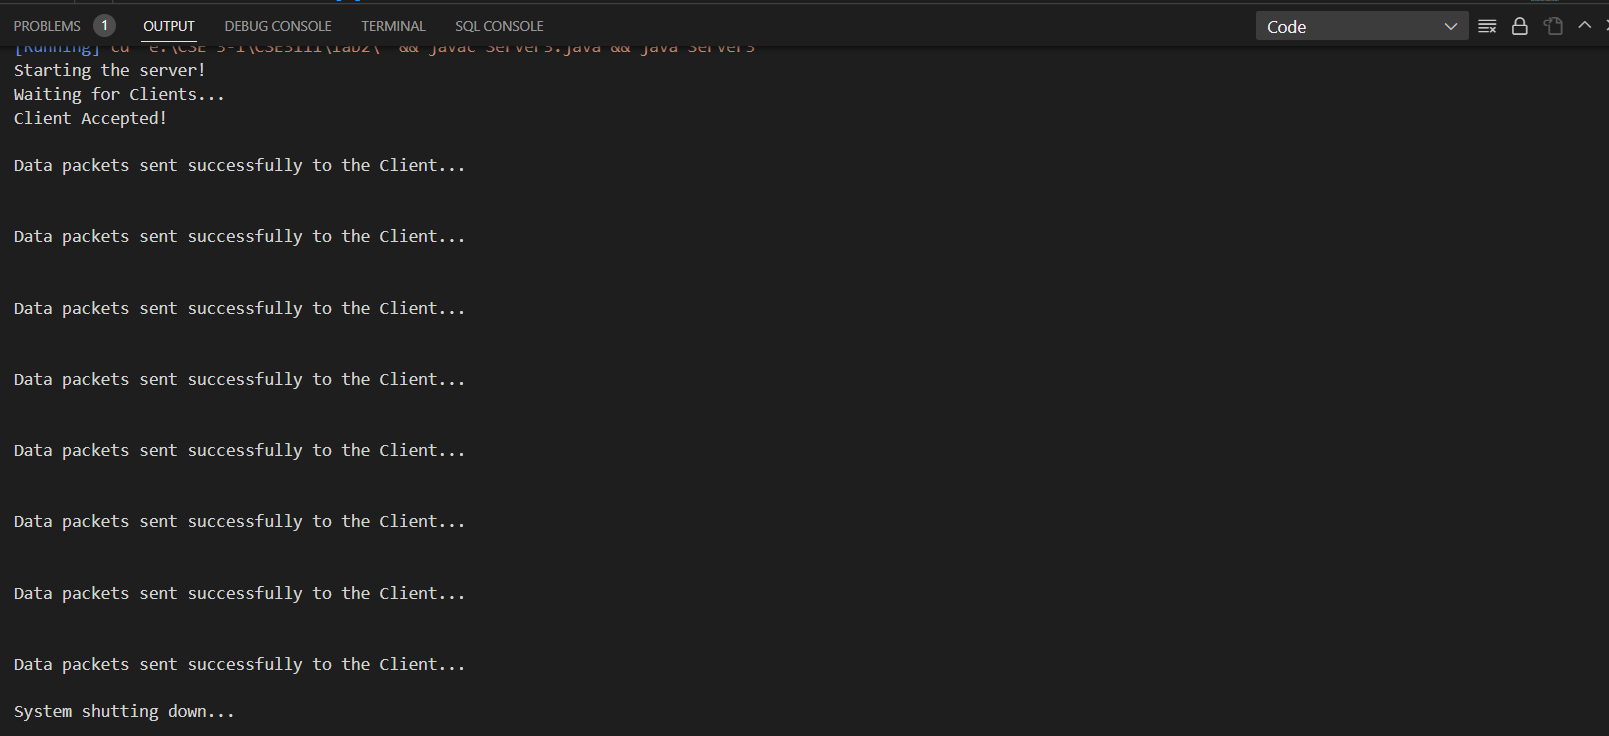
\includegraphics[width=\textwidth]{message_server.png}
\caption{Server Side For Handling Message Failures}
\end{figure}


\subsection{Handling Message Failure Requested By The Client - Client Side}
This part will handle the part of the registered clients login authentication . The logical part will ensure proper choice selection is used.
\lstinputlisting[language=java]{Client3.java}

\begin{figure}[!h]
\centering
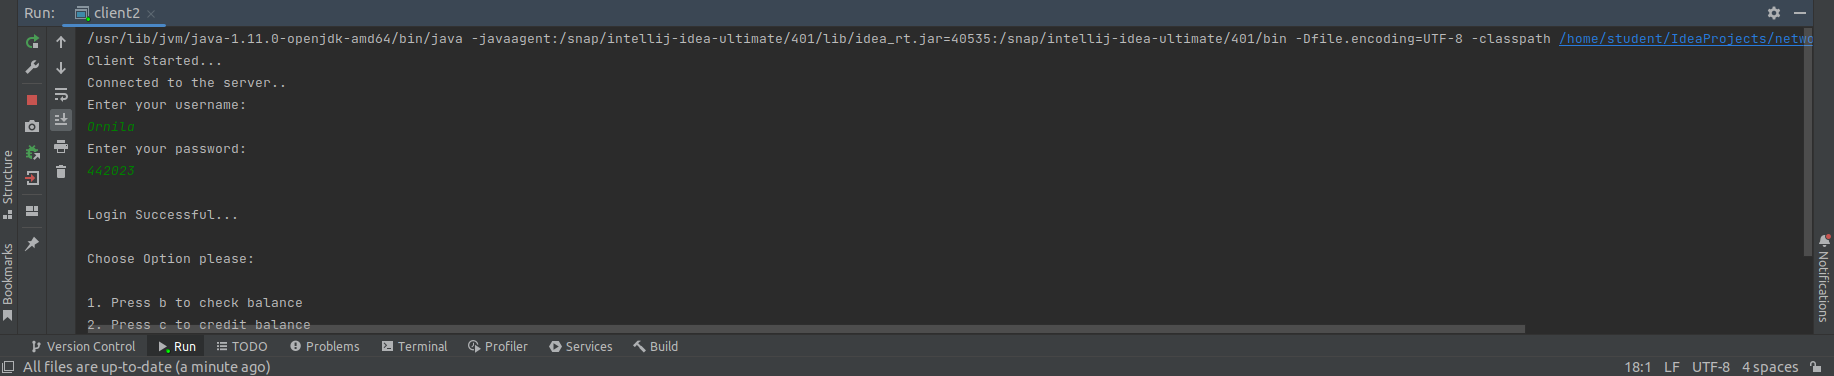
\includegraphics[width=\textwidth]{message1.png}
\caption{Client Side For Handling Message Failure}
\end{figure}
\begin{figure}[!h]
\centering
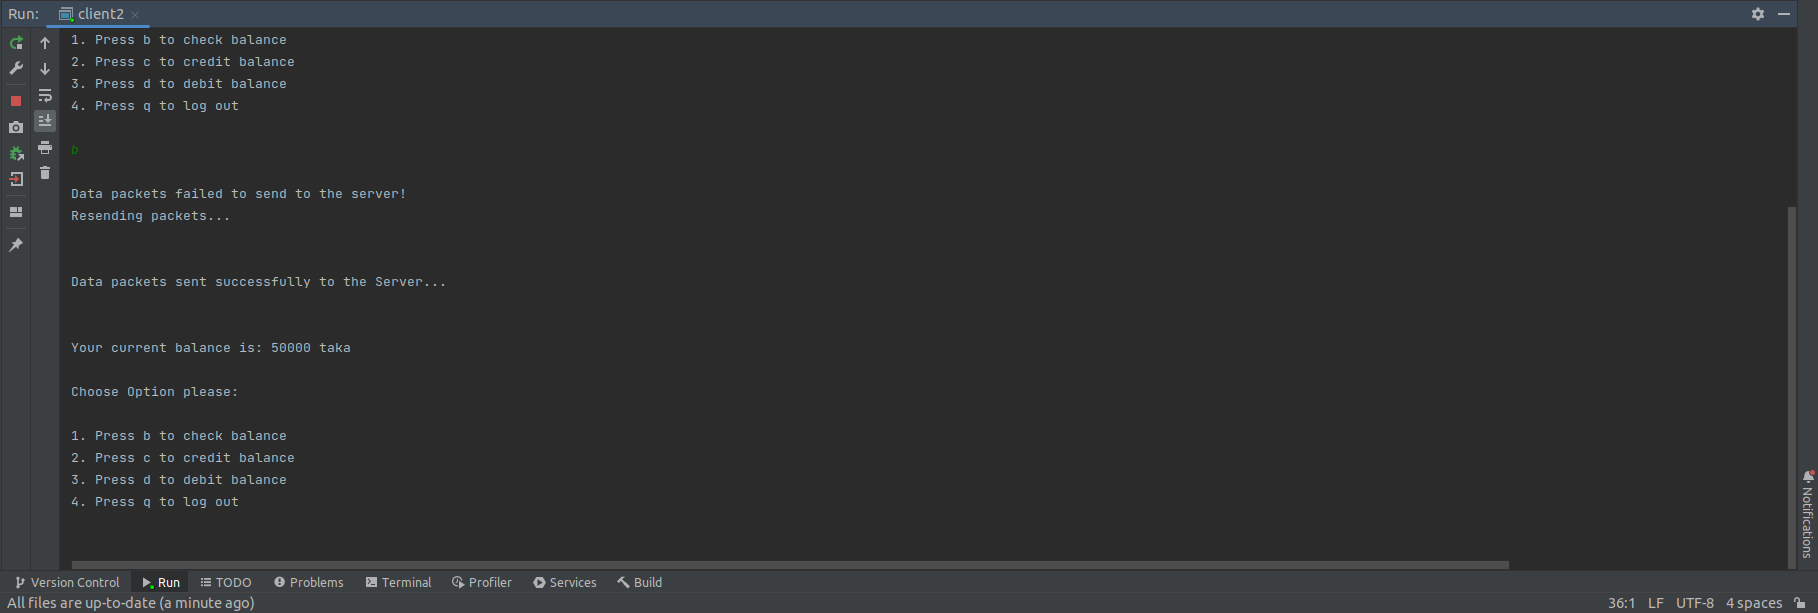
\includegraphics[width=\textwidth]{message2.png}
\caption{Client Side For Handling Message Failure}
\end{figure}

\begin{figure}[!h]
\centering
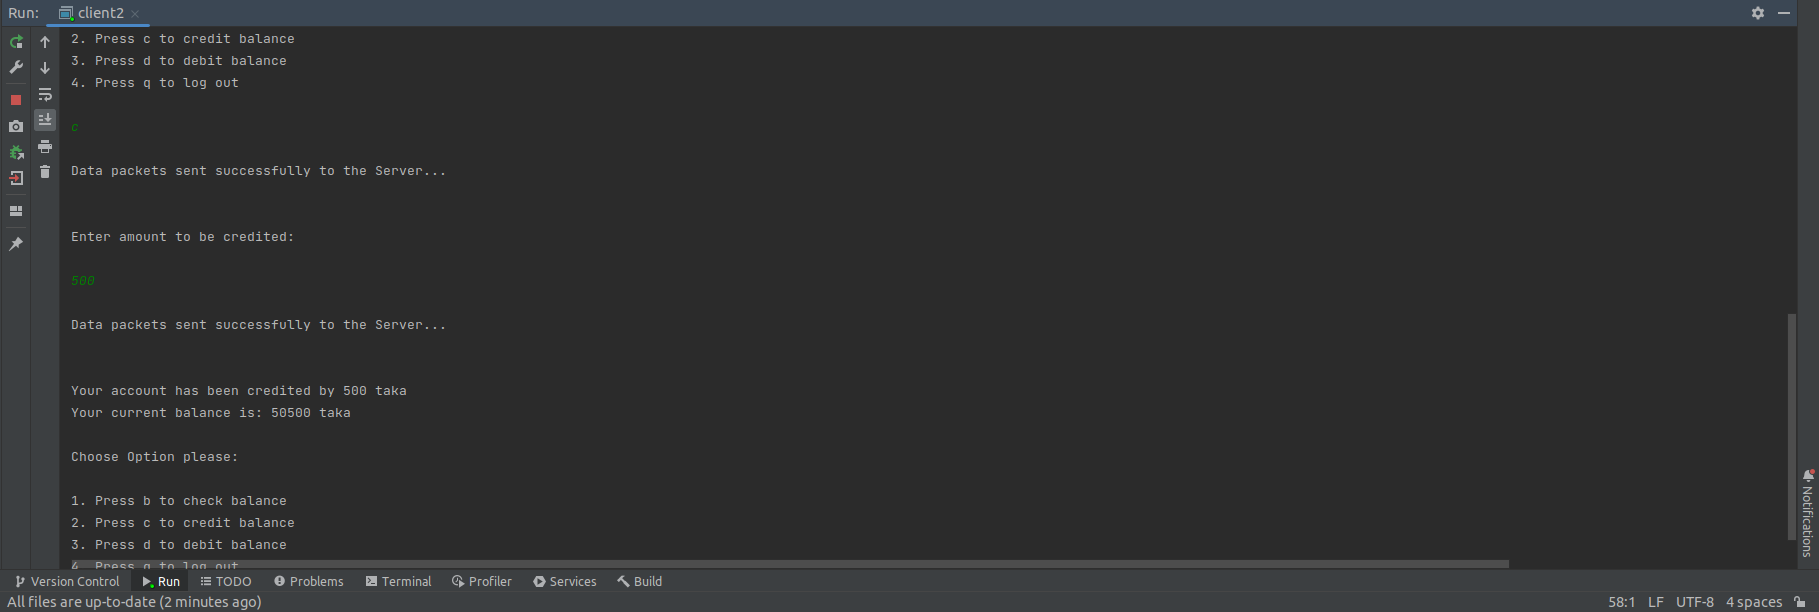
\includegraphics[width=\textwidth]{message3.png}
\caption{Client Side For Handling Message Failure}
\end{figure}
\begin{figure}[!h]
\centering
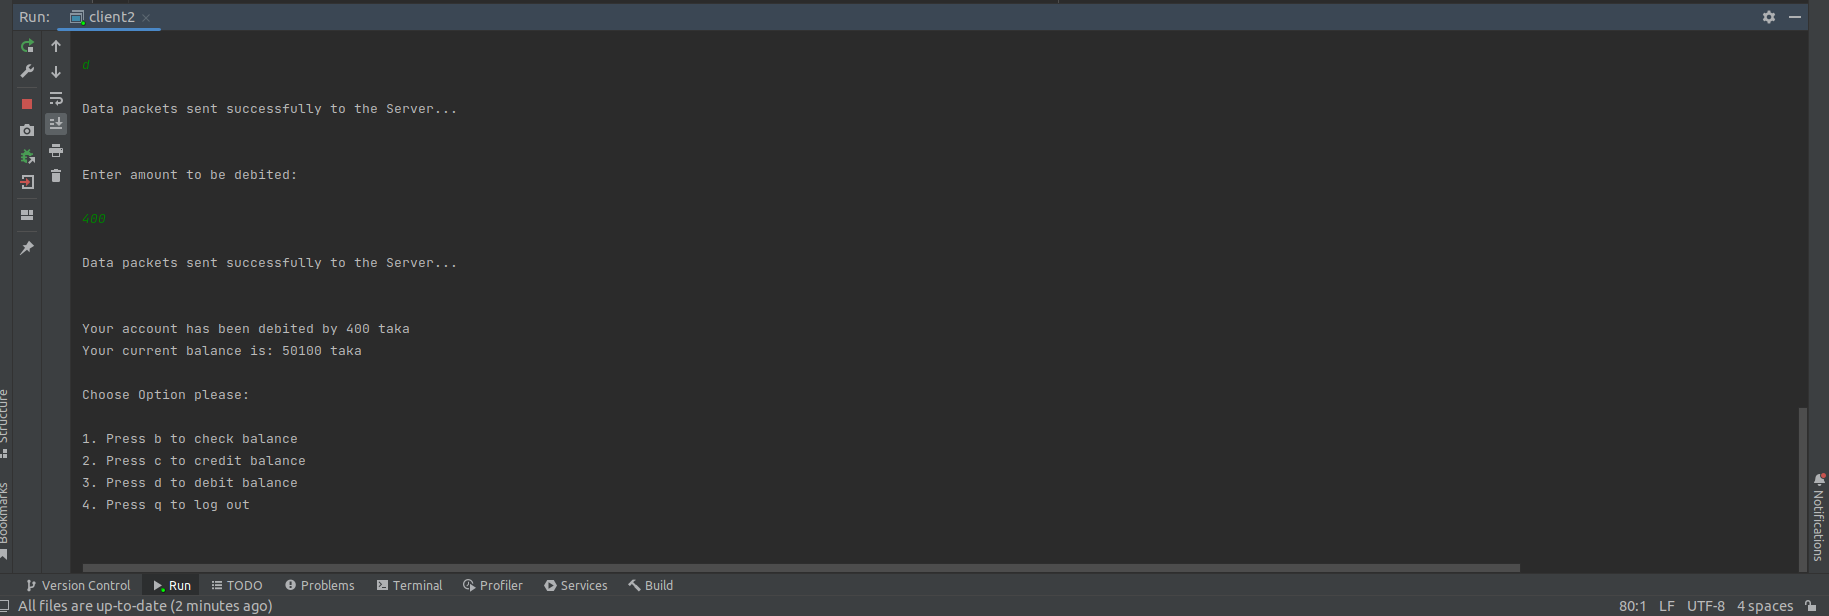
\includegraphics[width=\textwidth]{message4.png}
\caption{Client Side For Handling Message Failure}
\end{figure}
\begin{figure}[!h]
\centering
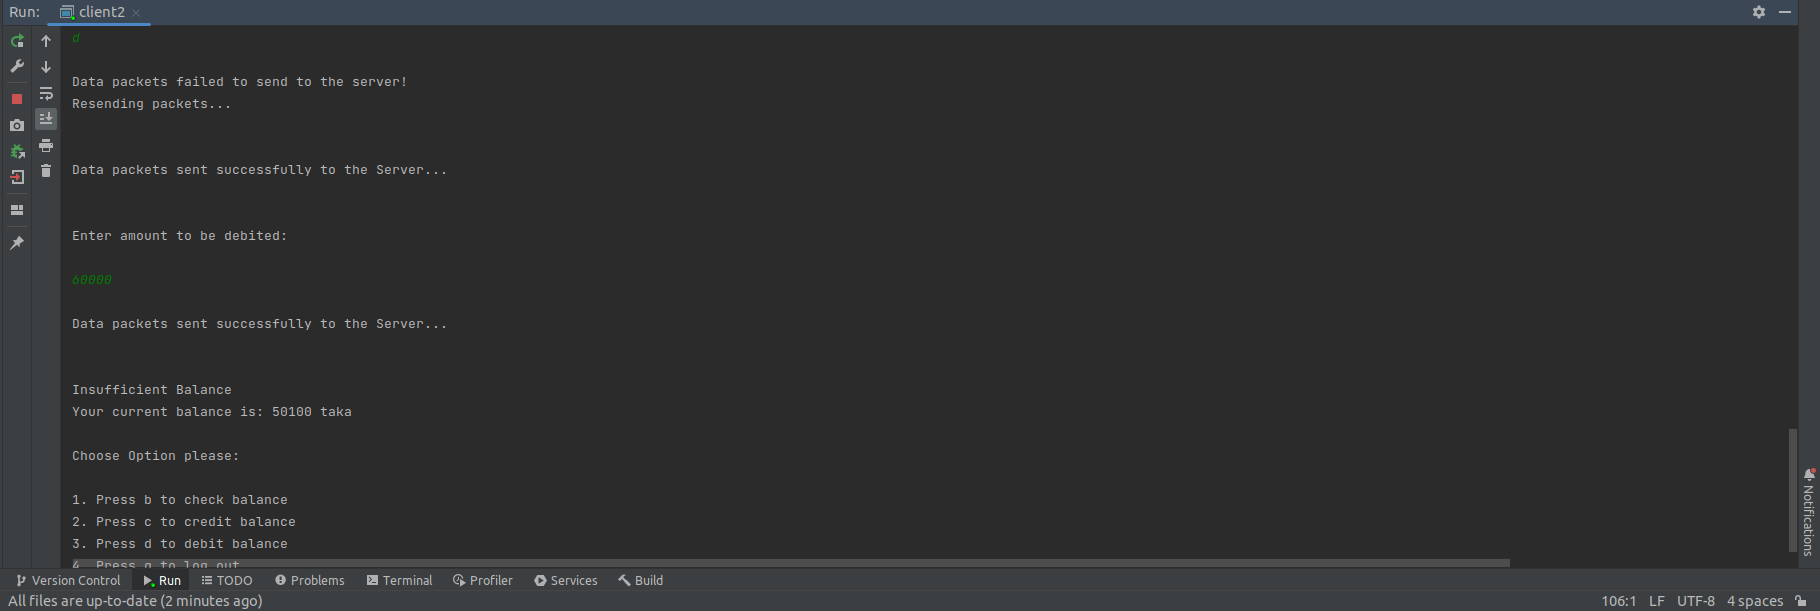
\includegraphics[width=\textwidth]{message5.png}
\caption{Client Side For Handling Message Failure}
\end{figure}
\begin{figure}[!h]
\centering
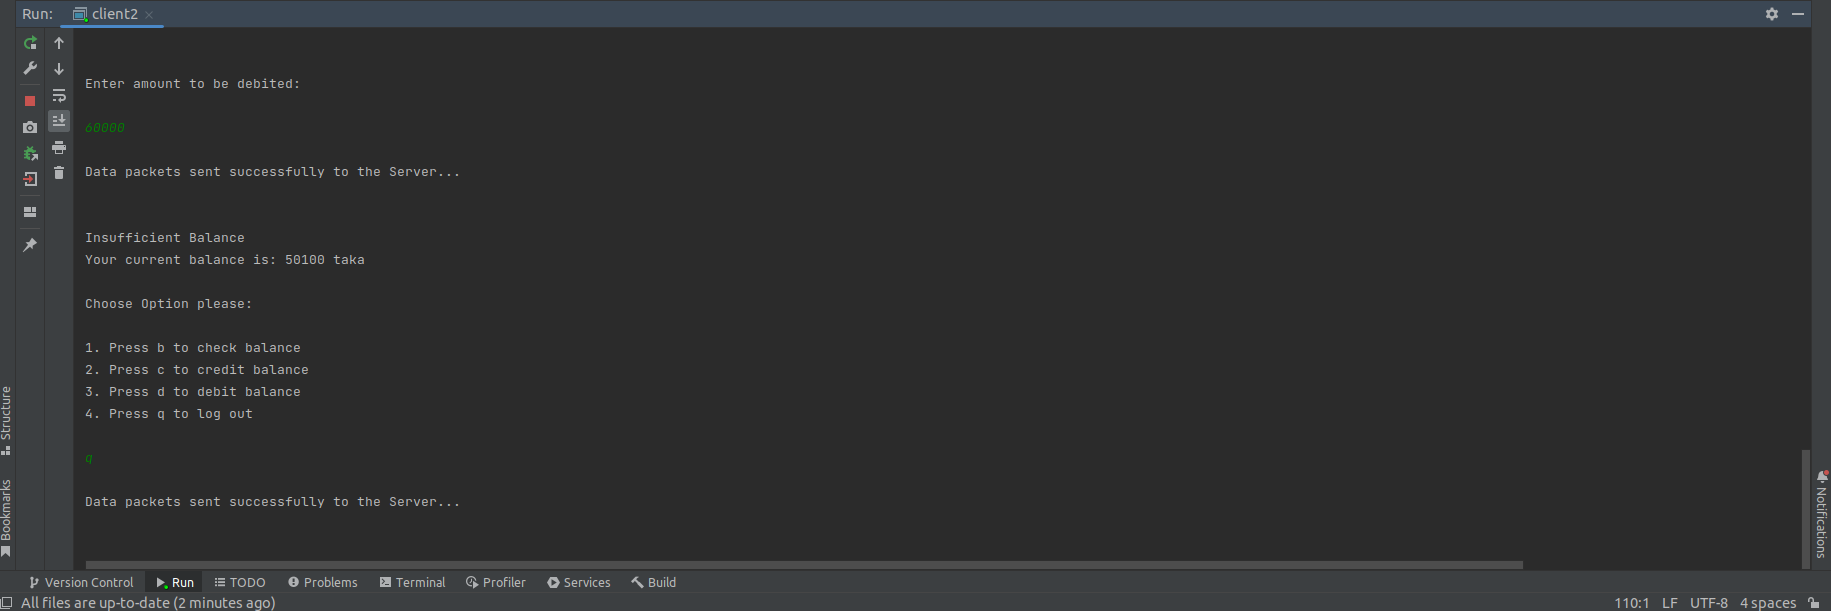
\includegraphics[width=\textwidth]{message6.png}
\caption{Client Side For Handling Message Failure}
\end{figure}



\newpage
\section{Experience}
\begin{enumerate}
\item We established a TCP connection between two hosts.
\item We used Java Programming Language to do Socket Programming in order to achieve basic information transfer between two hosts.
\end{enumerate}

\begin{thebibliography}{1}
\bibitem{book}  Computer networking : a top-down approach 6th ed.
\bibitem{GeeksForGeeks} GeeksForGeeks : \url{https://www.geeksforgeeks.org/socket-programming-in-java/}

\end{thebibliography}

\end{document}
